\chapter{STUDI DAN EKSPLORASI APACHE SPARK}
\label{chap:studi dan eksplorasi}

\section{Instalasi Apache Spark}

Pada bagian ini, akan dijelaskan tahap-tahap untuk melakukan instalasi Apache Spark. Apache Spark yang akan digunakan adalah Apache Spark versi x Spark dapat berjalan diatas berbagai sistem operasi seperti Window Windows dan UNIX systems (Contoh Linux, Mac OS). Sebelum memulai instalasi Apache Spark, ada beberapa kebutuhan yang harus dipenuhi seperti instalasi Java dan Scala. Berikut adalah langkah-langkah untuk memastikan kita telah memenuhi kebutuhan minimal:

\begin{itemize}

\item Pastikan bahwa Java telah diinstal dan versi java yang diinstall adalah setidaknya 8+ karena Spark berjalan pada versi minimal Java 8+. Berikut adalah command untuk memastikan java telah terinstall:

\begin{verbatim}
$ java -version

Java(TM) SE Runtime Environment (build 1.8.0_112-b15)                                                                   Java HotSpot(TM) 64-Bit Server VM (build 25.112-b15, mixed mode) 
\end{verbatim}


\item Pastikan bahwa Scala telah diinstal dengan versi minimal 2.11.x. Berikut adalah perintah untuk memastikan bahwa Scala telah terinstal dengan versi yang benar:

\begin{verbatim}
$ scala -version

Scala code runner version 2.11.6 -- Copyright 2002-2013, LAMP/EPFL
\end{verbatim}

\end{itemize} 

Bila Java dan Scala belum terinstal pada komputer, berikut adalah langkah-langkah instalasi Java dan Scala untuk kebutuhan Spark:

\begin{itemize}

\item Berikut adalah perintah-perintah untuk menginstal Java menggunakan terminal pada sistem operasi Linux:

\begin{verbatim}
$ sudo apt-get update
$ sudo apt-get install default-jdk
\end{verbatim}

\item Berikut adalah perintah-perintah untuk menginstal Scala menggunakan terminal pada sistem operasi Linux:

\begin{verbatim}
$ sudo apt-get update
$ sudo apt-get install scala
\end{verbatim}

\end{itemize}


Instalasi dapat dilakukan ketika syarat-syarat diatas telah dipenuhi. Berikut adalah langkah-langkah instalasi Apache Spark:

\begin{enumerate}

\item Pertama, donwload versi spark yang diinginkan  dari https://spark.apache.org/downloads.html

\item Kemudian, \textit{extract} Spark tar dengan command berikut:

\begin{verbatim}
$ cd /home/user/Downloads/ 
$ tar xvf spark-2.3.1-bin-hadoop2.7.tgz 
$ mv spark-2.3.1-bin-hadoop2.7 /home/user/spark-2.3.1-bin-hadoop2.7 
\end{verbatim}

\item Selanjutnya, kita harus menkonfigurasi \textit{environment variable} untuk Spark. Ubah file .bashrc dengan menambahkan perintah berikut pada file:

\begin{verbatim}
export SPARK_HOME=/home/user/spark-2.3.1-bin-hadoop2.7
export PATH=$PATH:/home/user/spark-2.3.1-bin-hadoop2.7/bin
\end{verbatim}

\item Terakhir jalankan perintah berikut untuk memastikan perubahan telah terjadi pada file .bashrc:

\begin{verbatim}
source .bashrc
\end{verbatim}

\item Ketika spark diinstall dengan benar, maka dengan perintah spark-shell kita dapat menjalankan spark-shell seperti pada (Gambar~\ref{fig:sparkshell}). Berikut adalah perintah untuk menjalankan spark-shell:

\begin{verbatim}
$ $SPARK_HOME/bin/spark-shell
\end{verbatim}

\begin{figure}[H]
    \centering  
    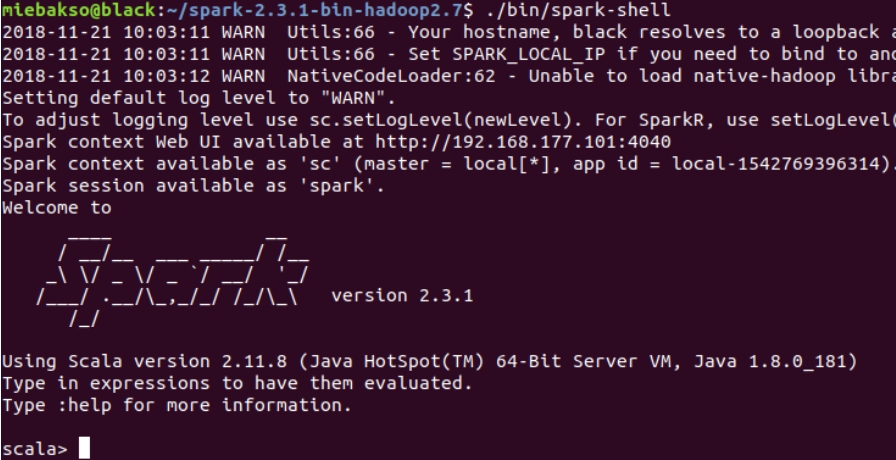
\includegraphics[scale=0.7]{sparkshell}  
    \caption[Gambar {\it Spark Shell} ]{Gambar {\it Spark Shell}} 
    \label{fig:sparkshell} 
\end{figure}

\end{enumerate}


\section{Eksplorasi Spark Shell}

Pada bagian ini, penulis akan menjelaskan percobaan untuk menghitung jumlah setiap kata pada file text README.md. Penulis akan menggunakan Spark Shell untuk menjalankan perintah-perintah agar spark bisa menghitung jumlah setiap kata yang ada pada text file tersebut. Setiap kata yang sama akan dijumlahkan. Pada bagian ini akan digunakan \textit{tranformation} dan juga \textit{action}.

\begin{figure}[H]
    \centering  
    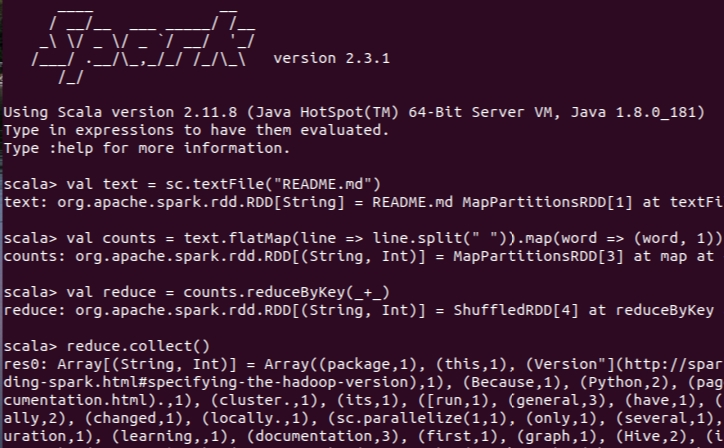
\includegraphics[scale=0.7]{wordcount}  
    \caption[Gambar {\it Word Count} ]{Gambar {\it Word Count}} 
    \label{fig:wordcount} 
\end{figure}

Bedasarkan gambar diatas (Gambar~\ref{fig:wordcount}), berikut adalah langkah-langkah percobaan:

\begin{enumerate}

\item Pertama, jalankan spark shell dengan command berikut pada terminal:

\begin{verbatim}
$ ./bin/spark-shell
\end{verbatim}

\item Setelah itu, kita akan membuat text RDD dari sumber eksternal yaitu file README.md. Command dibawah digunakan untuk membuat RDD dari file eksternal:

\begin{verbatim}
scala> val text = sc.textFile("README.md") 
\end{verbatim}

Dapat dilihat bahwa RDD bertipe \textit{String} telah sukses dibuat.

\begin{verbatim}
text: org.apache.spark.rdd.RDD[String] = README.md MapPartititonsRDD[1] at textFile at <console>:24
\end{verbatim}


\item Kemudian, kita akan memecahkan kalimat menjadi kata menggunakan operasi \textit{transformation} flatMap(). Setelah itu, setiap kata akan dijadikan pasangan textit{key} (kata) dan \textit{value} (kata,1). Berikut adalah perintah yang harus dijalankan:

\begin{verbatim}
val counts = text.textflatMap(line => line.split(" ")).map(word => (word, 1))
counts: org.apache.spark.rdd.RDD[(String, int)] = ShuffledRDD[3] ...
\end{verbatim}

\item Langkah selanjutnya, kita akan menghitung jumlah setiap kata dengan cara berikut. Operasi reduceByKey() akan menjumlahkan kata dengan \textit{key} yang sama. Contoh perintah dapat dilihat dibawah:  

\begin{verbatim}
val reduce = counts.reduceByKey(_+_)
reduce: org.apache.spark.rdd.RDD[(String, int)] = ShuffledRDD[4] ...
\end{verbatim}

\item Terakhir, kita akan mengambil hasil dengan perintah operasi collect() yang merupakan sebuah \textit{action}. Berikut adalah perintah yang harus dijalankan:

\begin{verbatim}
reduce.collect()
//Hasil
res0: Array[(String, Int)] = Array((package,1), (Python,2), .....
\end{verbatim}

\end{enumerate}

\section{Instalasi Apache Spark pada multi-node cluster}

Pada bagian ini, penulis akan menjelaskan langkah-langkah yang diperlukan untuk menginstal Spark pada\textit{ multi-node cluster}. Berikut adalah langkah-langkah yang harus dilakukan:

\begin{enumerate}

\item Tambahkan entri dalam file host \textit{master} dan \textit{slave}. \textit{Master} merupaka komputer utama dan \textit{slaves} merupakan komputer pekerja. Berikut adalah perintah yang harus dijalankan: 

\begin{verbatim}
$ sudo gedit /etc/hosts
\end{verbatim}

Tambahkan IP \textit{master} dan juga \textit{slave} pada file.

\begin{verbatim}
<MASTER-IP> master
<SLAVE1-IP> slave1
<SLAVE2-IP> slave2
<SLAVE3-IP> slave3
\end{verbatim}

\item Kemudian install Java pada setiap \textit{master} dan \textit{slave}, jangan lupa untuk memastikan versi java yang diinstall. Berikut adalah perintah untuk menginstal Java:

\begin{verbatim}
$ sudo apt-get update
$ sudo apt-get install default-jdk
\end{verbatim}

Pastikan versi Java yang diinstal dengan perintah berikut:

\begin{verbatim}
$ java -version
\end{verbatim}

\item Kemudian, instal Scala pada setiap master dan slave, jangan lupa untuk memastikan versi Scala yang diinstal.

\begin{verbatim}
$ sudo apt-get update
$ sudo apt-get install scala
\end{verbatim}

Pastikan veri Scala yang diinstal dengan perintah berikut:

\begin{verbatim}
$ scala -version
\end{verbatim}

\item Setelah melakukan instalasi Scala dan Java, maka kita perlu melakukan instalasi Open SSH Server-Client pada \textit{master}. Berikut adalah perintah yang harus dijalankan:

\begin{verbatim}
$ sudo apt-get install openssh-server openssh-client
$ ssh-keygen -t rsa -P 
\end{verbatim}

\item Selanjutnya, kita perlu melakukan konfigurasi SSH pada \textit{slave} dan juga \textit{master}. Salin \texttt{.ssh/id\_rsa.pub} miliki \textit{master} kepada \texttt{.ssh/authorized\_keys} untuk \textit{master} dan juga \textit{slave}.

\item Setelah itu, kita akan mengunduh dan menginstal Spark pada setiap \textit{slave} dan \textit{master}. Berikut adalah langkah-langkah yang diikuti:

\begin{verbatim}
Dowload versi spark yang diinginkan pada https://spark.apache.org/downloads.html

Extract spark dengan perintah berikut:

$ tar xvf spark-2.3.0-bin-hadoop2.7.tgz
$ sudo mv spark-2.3.0-bin-hadoop2.7 /home/user/spark
\end{verbatim}

\item Setelah selesai menginstal Spark, kita harus mengubah file .bashrc.

\begin{verbatim}
Buka file bashrc dengan command berikut:

$ sudo gedit .bashrc 

Tambahkan baris berikut pada file .bashrc:

export PATH = $PATH:/home/user/spark/bin

Jalankan perintah berikut untuk memastikan perubahan telah terjadi pada file .bashrc:

source .bashrc
\end{verbatim}

\item Kemudian, Spark harus dikonfigurasi untuk \textit{master} dengan mengubah file spark-env.sh. Berikut adalah perintah-perintah yang harus dijalankan

\begin{verbatim}
$ cd /home/user/spark/conf
$ cp spark-env.sh.template spark-env.sh
$ sudo gedit spark-env.sh

Tambahkan baris berikut pada file tersebut:

export SPARK_MASTER_HOST='<MASTER-IP>'
export JAVA_HOME=<Path_of_JAVA_installation>

Kemudian edit file slaves pada /home/user/spark/conf dengan perintah berikut:

$ sudo gedit slaves

Tambahkan baris berikut pada file tersebut:

master
slave1
slave2
slave3
\end{verbatim}

\item Sekarang, kita bisa menjalankan spark \textit{cluster} dengan perintah berikut:

\begin{verbatim}
$ cd /usr/local/spark
$ ./sbin/start-all.sh

Untuk memberhentikannya masukan perintah berikut:

$ ./sbin/start-all.sh
\end{verbatim}


\end{enumerate}

\section{Percobaan Spark Submit}

Pada percobaan ini, kita akan mecoba mengumpulkan sebuah jar kepada spark-submit. Aplikasi yang dibuat harus memiliki konfigurasi Spark dan diubah menjadi jar untuk dikumpulkan kepada spark-submit. Aplikasi yang dibuat akan membaca file yang disediakan dan menghitung jumlah kata yang ada. Sebelum melakukan percobaan, ada beberapa kebutuhan yang harus dipenuhi. Berikut adalah kebutuhan-kebutuhan yang harus dipenuhi:

\begin{enumerate}

\item Instal dan sudah melakukan konfigurasi untuk Scala, Java, dan Spark.

\item Instal IntelliJ IDEA dari https://www.jetbrains.com/idea/.

\item Install sbt, berikut adalah langkah instalasi sbt:

\begin{verbatim}
$ echo "deb https://dl.bintray.com/sbt/debian /" | sudo tee -a /etc/apt/sources.list.d/sbt.list
$ sudo apt-key adv --keyserver hkp://keyserver.ubuntu.com:80 --recv 2EE0EA64E40A89B84B2DF73499E82A75642AC823
$ sudo apt-get update
$ sudo apt-get install sbt
\end{verbatim}


\end{enumerate}

Setelah kebutuhan telah terpenuhi maka percobaan bisa dimulai. Berikut adalah langkah-langkah percobaan:

\begin{enumerate}

\item Pertama, buka Intelij dan buatlah sebuah project SBT seperti pada Gambar ~\ref{fig:intelij}.

\begin{figure}[H]
    \centering  
    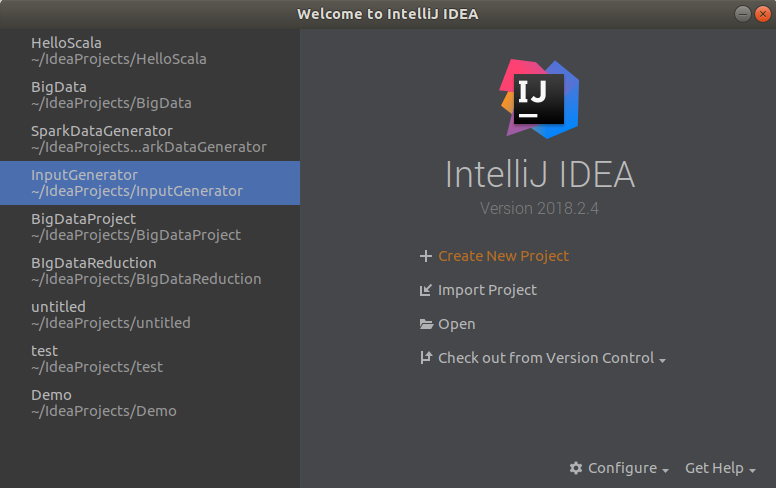
\includegraphics[scale=0.5]{intelij}  
    \caption[Gambar ItelliJ IDEA]{Gambar ItelliJ IDEA} 
    \label{fig:intelij} 
\end{figure}

Setelah itu, pilih proyek Scala yang menggunakan sbt. Tekan tombol \textit{next} seperti pada Gambar ~\ref{fig:newproject}.

\begin{figure}[H]
    \centering  
    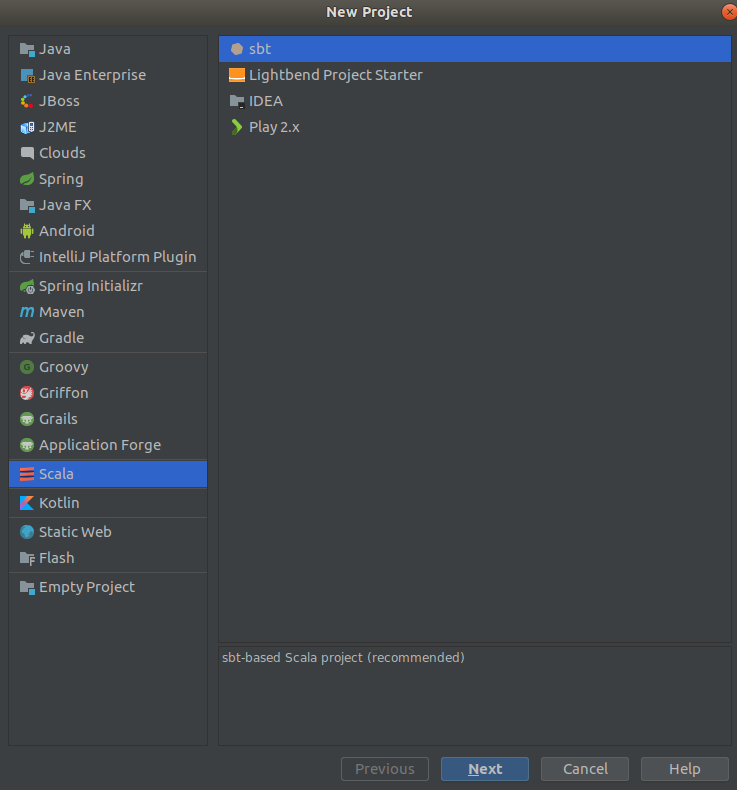
\includegraphics[scale=0.5]{newproject}  
    \caption[Gambar proyek sbt]{Gambar proyek sbt} 
    \label{fig:newproject} 
\end{figure}

Kemudian, namakan proyek dengan nama WordCount dan pilih versi sbt, java, dan scala yang sesuai seperti pada Gambar ~\ref{fig:projectconfig}. 

\begin{figure}[H]
    \centering  
    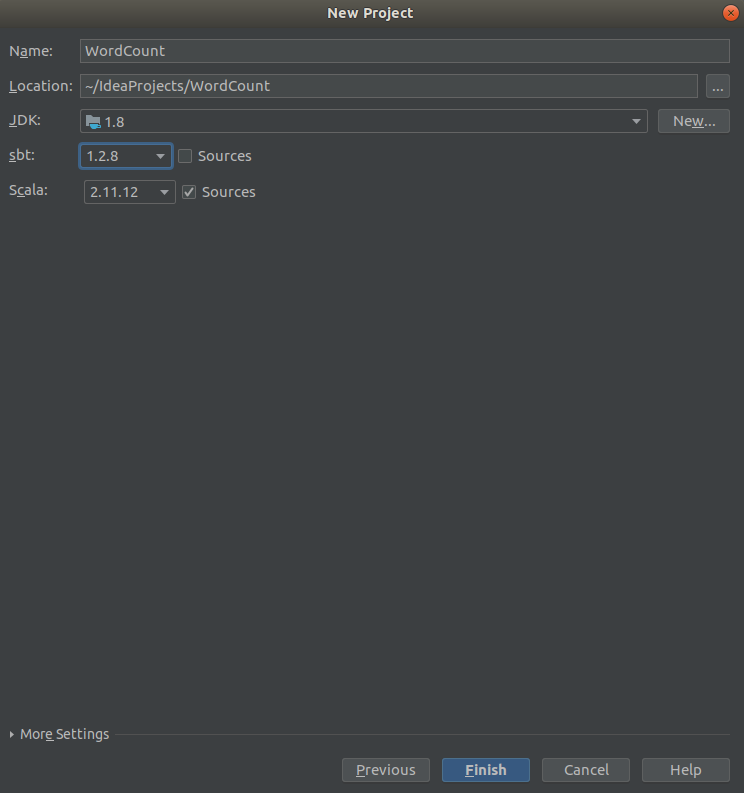
\includegraphics[scale=0.4]{projectconfig}  
    \caption[Gambar konfigurasi proyek]{Gambar konfigurasi proyek} 
    \label{fig:projectconfig} 
\end{figure}

Hasil dari pembuatan proyek baru pada IntelliJ akan terlihat seperti pada Gambar \ref{fig:structure}.

\begin{figure}[H]
    \centering  
    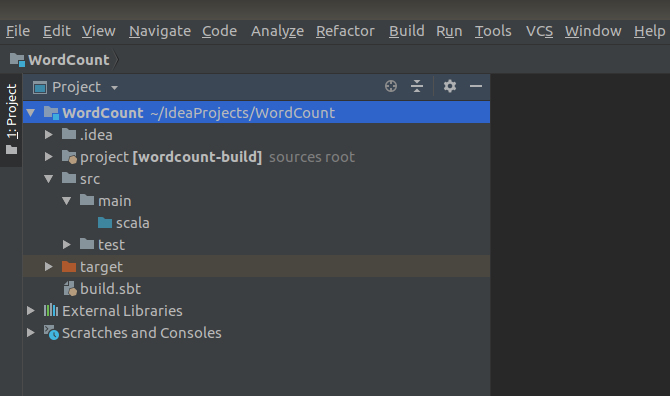
\includegraphics[scale=0.5]{structure}  
    \caption[Gambar struktur proyek ]{Gambar struktur proyek} 
    \label{fig:structure} 
\end{figure}

\item Setelah membuat proyek baru, buka file build.sbt dan tambahkan baris seperti pada Gambar \ref{fig:sbt}.


\begin{figure}[H]
    \centering  
    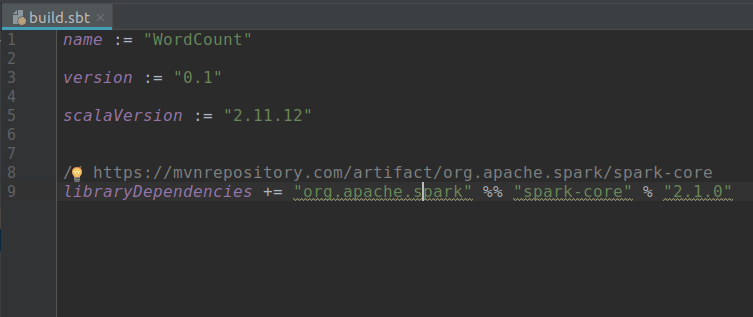
\includegraphics[scale=0.5]{sbt}  
    \caption[Gambar konfigurasi sbt]{Gambar konfigurasi sbt} 
    \label{fig:sbt} 
\end{figure}

\item Tambahkan \textit{object} WordCount pada proyek seperti pada Gambar \ref{fig:object}.

\begin{figure}[H]
    \centering  
    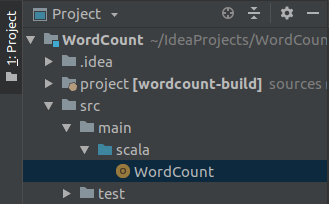
\includegraphics[scale=0.7]{object}  
    \caption[Gambar \textit{object} WordCount]{Gambar \textit{object} WordCount}.
    \label{fig:object} 
\end{figure}


Setelah itu, tambahkan kode berikut seperti pada Gambar \ref{fig:kodeword}.

\begin{figure}[H]
    \centering  
    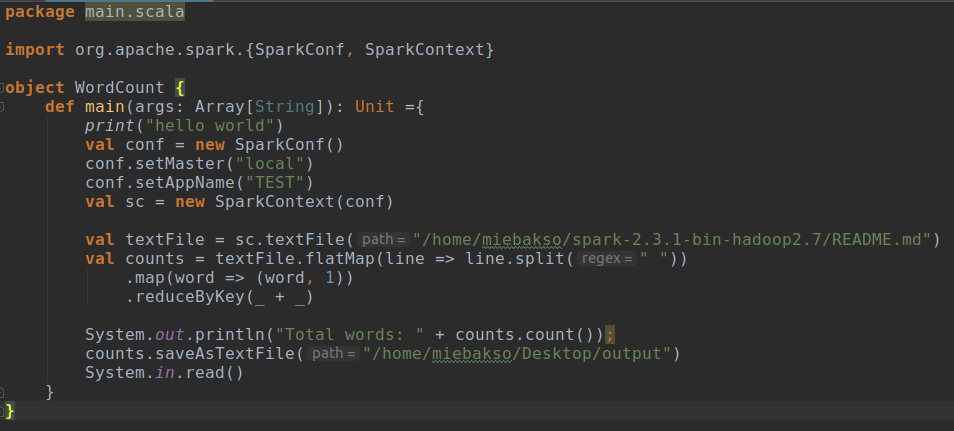
\includegraphics[scale=0.5]{kodeword}  
    \caption[Gambar kode WordCount]{Gambar kode WordCount} 
    \label{fig:kodeword} 
\end{figure}

\item Jalankan perintah 'sbt package' untuk meng-\textit{compile} kode menjadi \textit{executable} JAR seperti pada Gambar \ref{fig:jar}, hasil output dapat dilihat di Gambar \ref{fig:sbtpackage}.

\begin{figure}[H]
    \centering  
    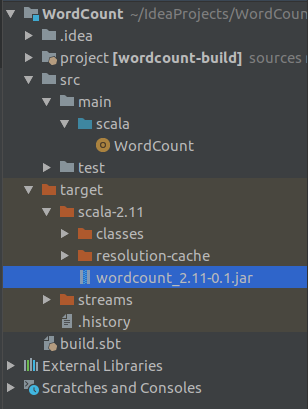
\includegraphics[scale=0.5]{jar}  
    \caption[Gambar JAR]{Gambar JAR} 
    \label{fig:jar} 
\end{figure}

\begin{figure}[H]
    \centering  
    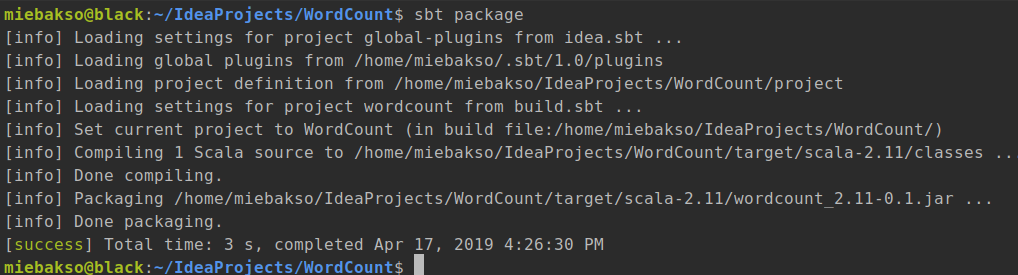
\includegraphics[scale=0.5]{sbtpackage}  
    \caption[Gambar hasil perintah 'sbt package']{Gambar hasil perintah 'sbt package'} 
    \label{fig:sbtpackage} 
\end{figure}

\item Setelah berhasil membuat JAR, kita akan memasukan file JAR kepada \textit{spark-submit} seperti pada Gambar \ref{fig:sparksubmit}. Berikut adalah perintah yang harus dijalankan: 

\begin{verbatim}
$ cd $SPARK_HOME
$ ./bin/spark-submit --class main.scala.WordCount --master local[1] \
/home/miebakso/IdeaProjects/WordCount/target/scala-2.11/wordcount_2.11-0.1.jar 
\end{verbatim}

\begin{figure}[H]
    \centering  
    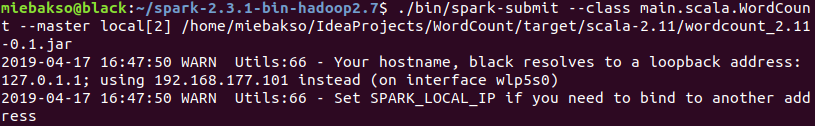
\includegraphics[scale=0.6]{sparksubmit}  
    \caption[Gambar penggumpulan JAR kepada \textit{spark-submit}]{Gambar penggumpulan JAR kepada \textit{spark-submit}} 
    \label{fig:sparksubmit} 
\end{figure}

Hasil tahap-tahap proses dari program dapat dilihat pada Spark UI dengan membuka alamat yang digaris bawah biru pada Gambar \ref{fig:linkui}

\begin{figure}[H]
    \centering  
    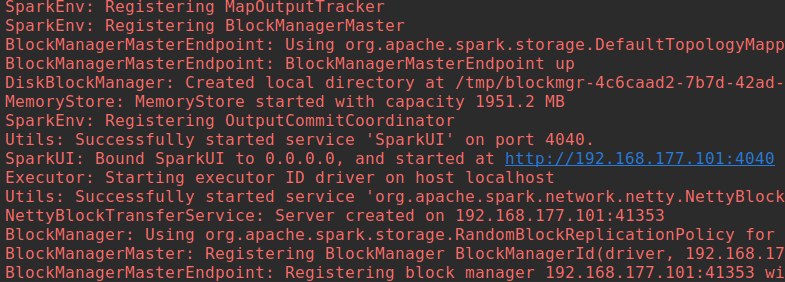
\includegraphics[scale=0.6]{linkui}  
    \caption[Gambar alamat Spark UI]{Gambar alamat Spark UI} 
    \label{fig:linkui} 
\end{figure}

Spark UI menggambarkan tahap-tahap proses program. Tampilan dari Spark UI dapat dilihat pada Gambar \ref{fig:sparkui}.
\begin{figure}[H]
    \centering  
    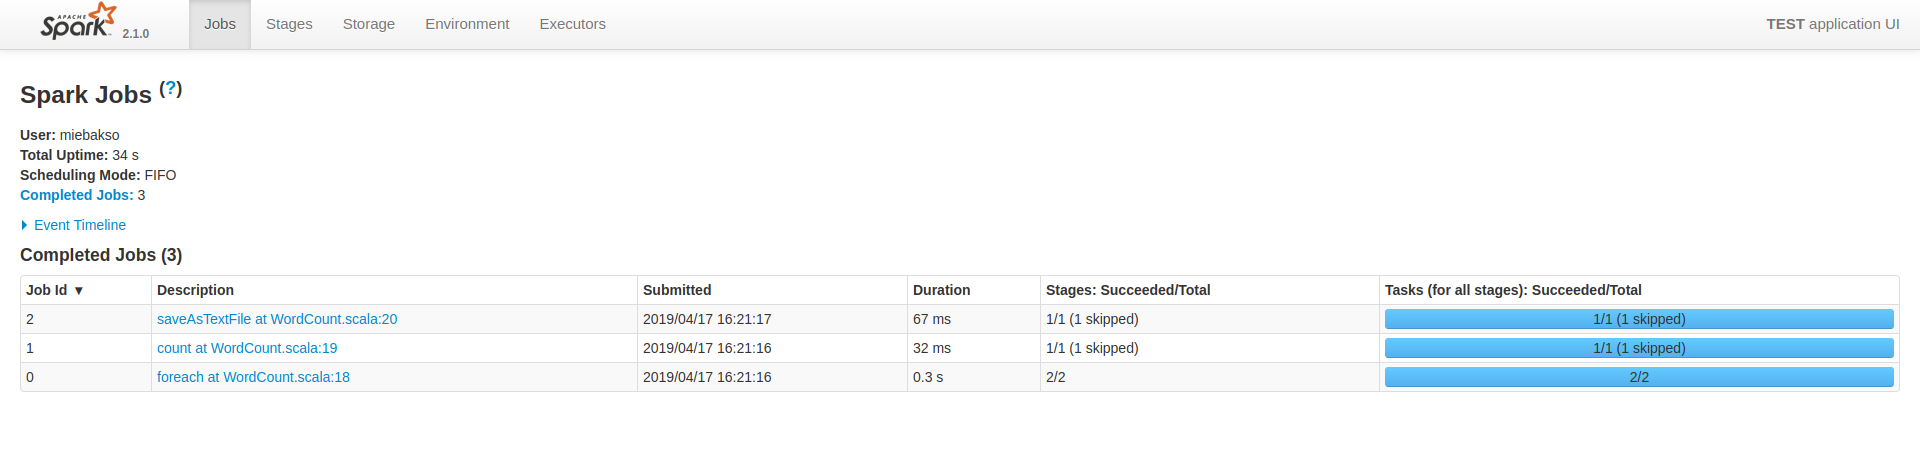
\includegraphics[scale=0.25]{sparkui}  
    \caption[Gambar Spark UI]{Gambar Spark UI} 
    \label{fig:sparkui} 
\end{figure}





 
\end{enumerate}
